\documentclass[conference,onecolumn]{IEEEtran}
\IEEEoverridecommandlockouts
% The preceding line is only needed to identify funding in the first footnote. If that is unneeded, please comment it out.
\usepackage{cite}
\usepackage{amsmath,amssymb,amsfonts}
\usepackage{algorithm,algorithmic}
\usepackage{graphicx}
\usepackage{textcomp}
\usepackage{xcolor}
\def\BibTeX{{\rm B\kern-.05em{\sc i\kern-.025em b}\kern-.08em
    T\kern-.1667em\lower.7ex\hbox{E}\kern-.125emX}}

% \documentclass{article}

\usepackage{hyperref} %BUG if put after
\usepackage{tikz}
\usetikzlibrary{calc,shapes,positioning}
\usetikzlibrary{arrows}
\newcommand{\midarrow}{\tikz \draw[-triangle 90] (0,0) -- +(.1,0);}
% Be sure to use PDxF Latex
\pdfoutput=1

% \usepackage[latin1]{inputenc}

\usepackage{url}
% \usepackage{fullpage}
\usepackage{cite}
% \usepackage{caption}
\usepackage{bm}
\newcommand{\ubar}[1]{\mkern2mu\underline{\mkern-2mu #1\mkern-2mu}\mkern2mu}
% \allowdisplaybreaks
\usepackage{mystyle}


\usepackage{amsmath,graphicx}
% format A4
% \usepackage{vmargin}
% \setpapersize{A4} 

\RequirePackage{algorithm}
\RequirePackage{algorithmic}

% Attempt to make hyperref and algorithmic work together better:
% \newcommand{\theHalgorithm}{\arabic{algorithm}}

\hypersetup{  
  bookmarks=true,
  backref=true,
  pagebackref=false,
  colorlinks=true,
  linkcolor=blue,
  citecolor=red,
  urlcolor=blue,
  pdftitle={alphaBP},
  pdfauthor={Dong Liu},
  pdfsubject={}
}

\captionsetup[figure]{labelformat={default},labelsep=period,name={Figure}}

\begin{document}
\title{$\alpha$ Belief Propagation as Fully Factorized Approximation}
\author{First Hand Scientists\\
  e-mail: doli@kth.se}
% \author{
% \IEEEauthorblockN{
% Dong Liu$^{1}$, Nima N. Moghadam$^{2}$, Lars~K. Rasmussen$^{1}$, Jinliang Huang$^{2}$, Saikat Chatterjee$^{1}$}

% \IEEEauthorblockA {$^{1}$ KTH Royal Institute of Technology, Stockholm, Sweden. }
% \IEEEauthorblockA {$^{2}$ Huawei Technologies Sweden AB, Stockholm, Sweden.}
% \IEEEauthorblockA{
% e-mail: \{doli, lkra, sach\}@kth.se, \{nima.najari.moghadam1, jinliang.huang\}@huawei.com}
% }



\maketitle
\begin{abstract}
  Belief propagation (BP) can do exact inference in loop-free graphs, but its performance could be poor in graphs with loops, and the understanding of its solution is limited.
  This work gives an interpretable belief propagation rule that is actually minimization of a localized $\alpha$-divergence. We term this algorithm as $\alpha$ belief propagation ($\alpha$-BP). % By $\alpha$-BP, any inference on a distribution $p$ is approximately answered by a fully factorized surrogate distribution $q$.
  The performance of $\alpha$-BP is tested in MAP (maximum a posterior) inference problems, where
  $\alpha$-BP can outperform (loopy) BP by a significant margin even in fully-connected graphs. 
  % \\
  % Choice2: This work follows Tom Minka's work and proposes a generalization for standard belief propagation (BP), which we denote by $\alpha$-BP. Similarly to BP, $\alpha$-BP can be interpreted as an approximate inference scheme in which an intractable distribution is approximated by a fully-factorized and tractable one. It is well-known that on non-sparse graphs conventional message passing algorithms such as loopy-BP almost always fails to converge. However, using numerical results in a linear system, we show that $\alpha$-BP can outperform BP by a significant margin even in a fully-connected graph. 
  
  % a fully factorized distribution to approximate an target distribution and  obtains $\alpha$ Belief Propagation ($\alpha$-BP), which generalizes standard BP. $\alpha$-BP can be interpreted as approximating a distribution $p$ by a fully factorized distribution $q$. Then the Bayesian inference problems on $p$ (usually computational expensive) can be approximately answered by relatively simple surrogate $q$. Message passing of $\alpha$-BP is obtained by a exemplified linear model. Numerical results on \textit{maximum a posterior} inference are reported.
\end{abstract}

\section{Introduction}\label{sec:introduction}
Bayesian inference provides a general mathematical framework for many learning tasks such as classification, denoising, object detection, and signal detection. The wide applications include but not limited to imaging processing \cite{zhang2013denoise}, multi-input-multi-output (MIMO) signal detection in digital communication \cite{cespedes2014ep,jeon2015optimality}, inference on structured lattice \cite{10.2307/25651244}, machine learning  \cite{2018arXiv180607066M, Lin:2015:DLM:2969239.2969280, yoon2019inferenceGraph}.
Specifically, statistic properties of a hidden variable $\bm{x} = \{x_1,\dots,x_N\}$ are of common interests in Bayesian inference. Practical interests usually include finding joint probability $p(\bm{x})$, marginal probability $p_i(x_i)$, the most probable state $\argmax_{\bm{x}} p(\bm{x})$. It can be extended to maximum a posterior (MAP) inference when it is conditional on some observation ($\argmax_{\bm{x}}p(\bm{x} | \cdot)$). Direct inference from $p(\bm{x})$ may be difficult computationally or technically. For instance, in the MAP inference problem, it could be the case that the gradient or subgradient of $p(\bm{x})$ may not exist and it is computationally prohibitive to search $\bm{x}$'s whole feasible space.


Probabilistic graphical models as structured graphs provide a framework for modeling the dependency between random variables. Belief propagation (BP) is a general message-passing algorithm for performing inference on graphical models. The intuition of BP is exchange of belief (statistical information) between neighboring nodes \cite{Bishop:2006:PRM:1162264}. When belief exchange converges, inference can be done by using the converged belief in graphical models. BP can solve inference problems exactly when the graphical model representation of $p(\bm{x})$ is loop-free or tree-structured \cite{kschischang2001factor_graph}.
When there are loops or circles in graphical models, BP is still a practical method to do inference approximately (loopy BP) by running it as if there is no loop. But its performance could be deteriorated significantly. In the loopy case,
there are attempts to study convergence properties of BP in special cases \cite{Ihler:2005:LBP:1046920.1088703, du2017convergenceBP}, but (loopy) BP may not converge in general.

Apart from the practical performance issues of BP in loopy graphs, the understanding of it is also limited. \cite{Yedidia:2000:GBP:3008751.3008848} shows that BP in loopy graphs approaches to a stationary point of an approximate free energy, the Bethe free energy in statistical physics. Based on this understanding, variants of BP are derived to improve BP. For instance, fractional BP in \cite{Wiegerinck:2002:FBP:2968618.2968673} applies a correction coefficient to each factor, generalized BP \cite{Yedidia:2000:GBP:3008751.3008848} propagates belief between different regions of a graph, and damping BP in \cite{Pretti2005damping} updates belief by combining old and new belief. Another track is expectation propagation (EP), introduced by Opper and Winther \cite{Opper:2000:GPC:1121900.1121911} and Minka \cite{Minka:2001:EPA:647235.720257, Minka:2001:FAA:935427}. In EP, a simpler factorized distribution defined in exponential distribution family is used to approximate the original complex distribution, and an intuitive factor-wise refinement procedure is used to find such an approximate distribution. The method has an intuition of minimizing a localized Kullback-Leibler (KL) divergence. This is discussed further in \cite{divergence-measures-and-message-passing} and it shows an unifying view of message passing algorithms. Following work stochastic EP \cite{yingzhen2015sep} explores its variant method for applications to large dataset.

In this work, we take the path of Minka's variational methods to improve BP and also to gain better understanding of BP in loopy graphs.
We define a surrogate distribution $q(\bm{x})$ first. $q(\bm{x})$ is assumed to be fully factorized and each factor of $q(\bm{x})$ represents a message in the factor graph representation of the original distribution $p(\bm{x})$. Fully factorization is the only requirement to $q(\bm{x})$. Then we define a message passing rule that is derived by minimizing a localized $\alpha$-divergence. This is factor-wise refinement of $q(\bm{x})$ iteratively. We refer to the obtained algorithm by $\alpha$-BP. The merits of $\alpha$ are as follows:
\begin{itemize}
\item[a.]{$\alpha$-BP has clear intuition as localized minimization of $\alpha$-divergence between original distribution $p$ and surrogate distribution $q$.}
\item[b.]{$\alpha$-BP generalizes the standard BP, since the message rule of BP is a special case of $\alpha$-BP.}
\item[c.]{$\alpha$}-BP could outperform BP significantly even in full-connected graphs while still maintaining simplicity of BP for inference. 
\end{itemize}

% It turns out the   Choice of $\alpha$ value affects the performance of $\alpha$-BP according our numerical results. $\alpha$-BP outperforms BP and MMSE in the exemplified linear model that is tested in our experiments this paper.

% -------------------------------------------------------

% Then try to minimize the information loss by using $q(\bm{x})$ to represent $p(\bm{x})$.  We follow Minka's work \cite{divergence-measures-and-message-passing} to make these steps feasible:
% \begin{itemize}
% \item Pick $q$ from a distribution family;
% \item Pick a divergence to measure the information loss due to use $q$ to represent $p$;
% \item Construct an optimization plan to approximate $p$ by $q$ with criteria of selected divergence;
% \item Propagate the optimization across factor graph.
% \end{itemize}
% Then we estimate the most probable $\bm{x}$ from $q(\bm{x})$.
% Fully factorized $q(\bm{x})$ is chosen such that we can avoid the search of whole discrete space $\Aa^{N}$. For the criteria selection, we use $\alpha$-divergence which generalize the classic Kullback-Leibler (KL) divergence. We refer to the obtained algorithm as $\alpha$-BP.


% When $\bm{x}$ is defined in unconstrained continuous space $\Rr^N$, the MAP inference problem may comes with closed-form solution. For instance, minimum mean square error (MMSE) in linear system. For cases where there is no closed-form solution, gradient decent based optimization methods \cite{DBLP:journals/corr/KingmaB14} could be applied to find the most probable $\bm{x}$ with target of maximizing the $p(\bm{x})$ (or log-likelihood) directly or using variational Bayesian \cite{DBLP:journals/corr/KingmaW13}.





% ---------------------------------------------------------------------
% Motivation starts from MRF and linear system, target to find most likely configuration/signal,
% 1. continuous support, $\Rr^n$, closed form or optimization algorithm
% 2. discrete finite support, no-closed form nor optimization method
% examples: compressed sensing, MIMO detection

% Introduction to graphical model and BP, this is usually used to cope with this problem here. Problem is the loopy graph, where performance is bad. Another problem is the leaf-root belief propagation explanation is gone loopy graph, since it is not tree structure any more.

% In this work, we attempt the problem via looking for fully factorized approximation to true posterior, by minimizing alpha-divergence in a heuristic fixed-point scheme. $\alpha$-BP It turns out this generalize the standard BP. \\
% 1. improvement can be achieved by alternating the choice of alpha value in $\alpha$-divergence. \\
% 2. Run $\alpha$-BP with prior belief from other low cost estimation, help further impove the configuration estimation.





\section{Preliminary}\label{sec:preliminary}
In this section, we provide the preliminaries that are needed in this paper. We introduce the $\alpha$-divergence and a graphical model that we are going to use to explain $\alpha$-BP.

\subsection{Divergence Measures}
As explained in Section~\ref{sec:introduction}, we are going to minimize $\alpha$-divergence between $p$ and $q$, which is defined as follows according to \cite{Zhu95informationgeometric}\cite{divergence-measures-and-message-passing}: \\
\begin{equation}\label{eq:alpha-divergence}
  \Dd_{\alpha}(p \| q ) = \frac{\int_{\bm{x}} \alpha p(\bm{x}) + (1-\alpha) q (\bm{x}) - p(\bm{x})^{\alpha} q(\bm{x})^{1-\alpha} d\bm{x}}{\alpha(1-\alpha)},
\end{equation}
where $\alpha$ is the parameter of $\alpha$-divergence, distribution $p$ and $q$ are unnormalized, i.e. $\int_{\bm{x}}p(\bm{x}) d\bm{x} \neq 1$, $\int_{\bm{x}}q(\bm{x}) d\bm{x} \neq 1$.

The classic KL divergence is defined as
\begin{equation}
  KL(p \| q) = \int p(\bm{x}) \log{\frac{p(\bm{x})}{q(\bm{x})}} d \bm{x}+ \int q(\bm{x}) - p(\bm{x}) d\bm{x}
\end{equation}
where the $\int q(\bm{x}) - p(\bm{x}) d\bm{x}$ is a correction factor to accommodate unnormalized $p$ and $q$. The KL divergence is a special case of $\alpha$-divergence, since $\lim_{\alpha \rightarrow 1}\Dd_{\alpha}(p \| q ) = KL(p\|q)$ and $\lim_{\alpha \rightarrow 0}\Dd_{\alpha}(p \| q ) = KL(q\|p)$, by applying L'H\^opital's rule to \autoref{eq:alpha-divergence}.

Both $\alpha$-divergence and KL divergence are equal to zero if $p=q$, and they are non-negative (therefore satisfy the basic property of error measure).
Denote KL-projection by
\begin{equation}
  \text{proj}[p] = \uargmin{q \in \Ff} KL(p\|q),
\end{equation}
where $\Ff$ is the distribution family of $q$.

According to the stationary point equivalence Theorem in \cite{divergence-measures-and-message-passing}, $\text{proj}[p^{\alpha}q^{1- \alpha}]$ and $\Dd_{\alpha}(p\|q)$ have same stationary points. A heuristic scheme to find $q$ minimizing $\Dd_{\alpha}(p\|q)$ is to find its stationary point by a fixed-point iteration:
\begin{equation}\label{eq:fixed-point-iter}
  q(\bm{x})^{\text{new}}  = \text{proj}[p(\bm{x})^{\alpha}q(\bm{x})^{1-\alpha}].
\end{equation}

\subsection{A Graphic Model}

\begin{figure}
  \begin{centering}
    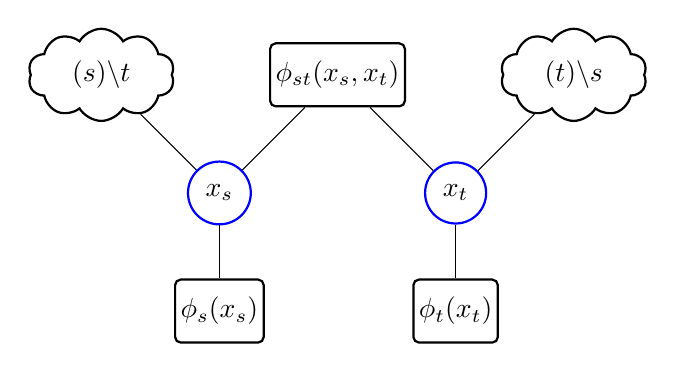
\begin{tikzpicture}
      % \tikzstyle{enode} = [thick, draw=blue, circle, inner sep = 3pt,
      % align=center]
      \tikzstyle{enode} = [thick, draw=blue, circle, inner sep = 4pt,  align=center]
      \tikzstyle{nnode} = [thick, rectangle, rounded corners = 2pt,minimum size = 0.8cm,draw,inner sep = 2pt]

      \tikzstyle{cnode} = [thick, cloud, draw,cloud puffs=10, cloud puff arc=120, aspect=2, inner ysep=4pt]

      \node[cnode] (pajk) at (3, 1.5) {$\Nn(t)\backslash s$};
      \node[cnode] (paik) at (-3, 1.5) {$\Nn(s)\backslash t$};

      \node[nnode] (tk) at (0, 1.5) {$\phi_{st}(x_s, x_t)$};
      \node[enode] (xi) at (-1.5 ,0) {$x_s$};
      \node[nnode] (fi) at (-1.5 , -1.5) {$\phi_s(x_s)$};

      \node[enode] (xj) at (1.5 ,0) {$x_t$};
      \node[nnode] (fj) at (1.5 , -1.5) {$\phi_t(x_t)$};
      % connections

      \draw[-] (xi) to (fi);
      \draw[-] (xi) to (tk);
      \draw[-] (xi) to (paik);

      \draw[-] (xj) to (fj);
      \draw[-] (xj) to (tk);
      \draw[-] (xj) to (pajk);
    \end{tikzpicture}
    \caption{Factor graph illustration of \autoref{eq:mrf}.}\label{fig:factor-graph}
    \vspace{0.1cm}
  \end{centering}
\end{figure}
We introduce a pairwise Markov random field (MRF) $p(\bm{x})$ to
explain our algorithm. Variable $\bm{x} := \left\{ x_1, x_2, \cdots,
  x_N \right\}$, where $x_i \in \Aa$ is a discrete finite set or subset of
$\RR$, and $N$ is a positive integer.
An undirected graphical model, known as Markov random field, defines a
family of joint probability distributions over $\bm{x}$ by associating
its index set with the vertex set $\Vv$ of undirected graph
$\Gg:=(\Vv, \Ee)$. The graph contains edges $\Ee \subset \Vv \times
\Vv$, where a pair of $(s, t) \in \Ee$ if and only if nodes $v$ and
$u$ are connected by a edge. For a clique $\Cc$ of the graph, let
$\phi_{\Cc}: \Aa^{\abs{\Cc}} \rightarrow (0, \infty)$ be a potential
function of vector $\bm{x}_{\Cc}:=\left\{ x_v| v\in \Cc \right\}$. Let
us then write the joint distribution of $\bm{x}$ as
\begin{equation}\label{eq:mrf}
  p(\bm{x}) \propto \prod_{{s\in \Vv}} \phi_s(x_s) \prod_{(s,t) \in \Ee} \phi_{st}(x_s, x_t),
\end{equation}
where $\propto$ denotes the fact that the only difference between two sides of $\propto$ is a constant factor.

The factor graph representing \autoref{eq:mrf} is shown in
\autoref{fig:factor-graph}. In the figure, $\Nn(s)$ is the node set of
pairwise factors connecting to variable node $x_s$, and $\backslash$ denotes exclusion.

\section{$\alpha$-BP with Fixed Global $\alpha$}\label{sec:alpha-bp-factor-refine}
In this section, we will show why $\alpha$-BP as a message-passing algorithm can be used as a fully-factorized approximation to the original distribution $p(\bm{x})$. 




\subsection{$\alpha$ Belief Propagation}\label{sec:alpha-bp-a}
\subsubsection{Fully Factorized Surrogate}
Now we formulate a surrogate distribution as
\begin{equation}
  q(\bm{x}) \propto \prod_{{s\in \Vv}} \tilde{\phi}_s(x_s) \prod_{(s,t) \in \Ee} \tilde{\phi}_{st}(x_s, x_t),
\end{equation}
to approximate $p(\bm{x})$. The surrogate distribution would be used to estimate inference problems of $p(\bm{x})$. We further assume that $q(\bm{x})$ can be fully factorized, which means that $\tilde{\phi}_{s,t}(x_s, x_t)$ can be factorized as two independent functions of $x_s, x_t$ respectively. We denote this factorization as
\begin{equation}
  \tilde{\phi}_{s,t}(x_s, x_t) := m_{st}(x_t) m_{ts}(x_s).
\end{equation}
We use the notation $m_{ts}(x_s)$ to denote the factor as a function of $x_s$ due to the intuitive fact that $m_{ts}$ is also the message from the factor $\phi_{ts}(x_t, x_s)$ to variable node $x_s$. Similarly we have factor $m_{st}(x_t)$. Then the marginal can be formulated straightforwardly as
\begin{equation}
  q_s(x_s) \propto \tilde{\phi}_s(x_s) \prod_{w\in \Nn(s)} m_{ws}(x_s).
\end{equation}

\subsubsection{Local $\alpha$-Divergence Minimization}

Now, we are going to use the heuristic scheme as in \autoref{eq:fixed-point-iter} to minimize the information loss by using tractable $q(\bm{x})$ to represent $p(\bm{x})$. The information loss is measured by $\alpha$-divergence $\Dd_{\alpha}(p(\bm{x}) \| q(\bm{x}))$.

We do factor-wise refinement to update the factors of $q(\bm{x})$ such that $q(\bm{x})$ approaches $p(\bm{x})$ asymptotically similar to \cite{divergence-measures-and-message-passing,Minka:2001:EPA:647235.720257}. Without losing generality, we begin to refine factor $\tilde{\phi}_{ts}(x_t, x_s)$. When doing the refinement of factor $\tilde{\phi}_{ts}(x_t, x_s)$, parameter $\alpha_{ts}$ is used. Define $q^{\backslash (t,s)}(\bm{x})$ as all other factors except for $\tilde{\phi}_{ts}(x_t, x_s)$
\begin{align}
  q^{\backslash (t,s)}(\bm{x})
  &= q(\bm{x})/\tilde{\phi}_{ts}(x_t,
    x_s) \nonumber \\
  &\propto \prod_{{s\in \Vv}} \tilde{\phi}_s(x_s) \prod_{(v,u) \in
    \Ee\backslash (t,s)}
    \tilde{\phi}_{vu}(x_v, x_u) \nonumber \\
  &= \left(
    \tilde{\phi}_s(x_s) \prod_{w\in \Nn(s) \backslash t}m_{ws}(x_s)
    \right)
    \left(
    \tilde{\phi}_t(x_t) \prod_{w\in \Nn(t) \backslash s}m_{wt}(x_t)
    \right)
    \left(
    \prod_{v \in \Vv \backslash s,t}
    \tilde{\phi}_v(x_v) \prod_{w\in \Nn(v)}m_{wv}(x_v)
    \right)\nonumber \\
\end{align}
Similarly, we have $p^{\backslash (t,s)}(\bm{x})$ as all other factors except for ${\phi}_{ts}(x_t, x_s)$. Assume that we already have had $q^{\backslash (t,s)}(\bm{x})$ as a good approximation of $p^{\backslash (t,s)}(\bm{x})$, i.e. $q^{\backslash (t,s)}(\bm{x}) \simeq p^{\backslash (t,s)}(\bm{x})$, it is $\tilde{\phi}_{ts}(x_t, x_s)$ that remains to be refined. 
Then the problem $\uargmin{\tilde{\phi}_{ts}^{\mathrm{new}}} \Dd_{\alpha_{ts}}\left(  p^{\backslash (ts)}\phi_{ts}\|q^{\backslash (t,s)}\tilde{\phi}_{ts}^{\mathrm{new}}\right)$ becomes \vspace{-0.3cm}
\begin{equation}\label{eq:alpha-minimize-factor}
  \uargmin{\tilde{\phi}_{ts}^{\mathrm{new}}(x_t, x_s)}
  \Dd_{\alpha_{ts}}\left( q^{\backslash (t,s)}(\bm{x}){\phi}_{ts}(x_t, x_s)
    \|q^{\backslash (t,s)}(\bm{x})\tilde{\phi}_{ts}^{\mathrm{new}}(x_t, x_s) \right),
\end{equation}
which searches for new factor $\tilde{\phi}_{ts}^{\mathrm{new}}(x_t, x_s)$ such the above divergence is minimized.
Using \autoref{eq:fixed-point-iter}, the above problem is equivalent to
\begin{align}\label{eq:update-rule}
  &q^{\backslash (t,s)}(\bm{x})\tilde{\phi}_{ts}^{\mathrm{new}}(x_t, x_s)  \nonumber\\
  &\propto \text{proj}\left[ \left( q^{\backslash (t,s)}(\bm{x}){\phi}_{ts}(x_t, x_s) \right)^{\alpha_{ts}} \left(q^{\backslash (t,s)}(\bm{x})\tilde{\phi}_{ts}(x_t, x_s)  \right)^{1-\alpha_{ts}} \right] \nonumber \\
  & \propto \text{proj}\left[ q^{\backslash
    (t,s)}(\bm{x}){\phi}_{ts}(x_t, x_s)^{\alpha_{ts}} \tilde{\phi}_{ts}(x_t, x_s)^{1-\alpha_{ts}} \right].
\end{align}

Let us refine one message per time on edge $(t,s)$. Without lose of generality, we update $m_{ts}$ and denote
\begin{equation}
  \tilde{\phi}_{ts}^{\mathrm{new}}(x_t, x_s) = m_{ts}^{\mathrm{new}}(x_s) m_{st}(x_t).
\end{equation}
Since KL-projection to a fully factorized distribution reduces to matching the marginals, \autoref{eq:update-rule} is reduced to
\begin{equation}\label{eq:message-update}
  \sum_{\bm{x}\backslash x_s} q^{\backslash (t,s)}(\bm{x}) \tilde{\phi}_{ts}^{\mathrm{new}}(x_t, x_s) \propto \sum_{\bm{x}\backslash x_s} q^{\backslash (t,s)}(\bm{x}) \phi_{ts}(x_t, x_s)^{\alpha_{ts}} \tilde{\phi}_{ts}(x_t, x_s)^{1-\alpha_{ts}}.
\end{equation}
We use summation here. But it should be replaced by integral if $\Aa$ is a continuous set.
Solving \autoref{eq:message-update} gives the message passing rule as
\begin{equation}\label{eq:message-rule}
  {m}^{\text{new}}_{ts}(x_s) \propto  m_{ts}(x_s)^{1-\alpha_{ts}} \bigg[
  \sum_{x_t} \phi_{ts}(x_t, x_s)^{\alpha_{ts}} {m}_{st}(x_t)^{1-\alpha_{ts}}
  \tilde{\phi}_t(x_t) \prod_{w\in \Nn(t)\backslash s}m_{wt}(x_t) \bigg].
\end{equation}

As for the singleton factor $\tilde{\phi}_t(x_t)$, we can do the refinement procedure on $\tilde{\phi}_t(x_t)$ in the same way as we have done for $\tilde{\phi}_{ts}(x_t, x_s)$. This gives us the update rule of $\tilde{\phi}_t(x_t)$ as
\begin{equation}\label{eq:fix-factor-update}
  \tilde{\phi}_t^{\mathrm{new}}(x_t) \propto \phi_t(x_t)^{\alpha_{t}} \tilde{\phi}_t(x_t)^{1-\alpha_{t}},
\end{equation}
which is the belief from factor $\phi_t(x_t)$ to variable $x_t$. Here $\alpha_t$ is the $\alpha$ value of $\alpha$-divergence in approximating factor $\phi_t(x_t)$. Note, if
we initialize $\tilde{\phi}_t(x_t) = \phi_t(x_t)$, then it remains the
same in all iterations, which makes
\begin{equation}\label{eq:message-rule}
  {m}^{\text{new}}_{ts}(x_s) \propto  m_{ts}(x_s)^{1-\alpha_{ts}} \bigg[
  \sum_{x_t} \phi_{ts}(x_t, x_s)^{\alpha_{ts}} {m}_{st}(x_t)^{1-\alpha_{ts}} {\phi}_t(x_t) \prod_{w\in \Nn(t)\backslash s}m_{wt}(x_t) \bigg].
\end{equation}
For factor notations, $\phi_{ts}=\phi_{st}$. We associated each factor with a $\alpha$ value, which gives us $\alpha_{ts} = \alpha_{st}$.


\subsection{Remarks on $\alpha$-BP}\label{subsec:remark}
\begin{figure}[!ht]
  \begin{centering}
    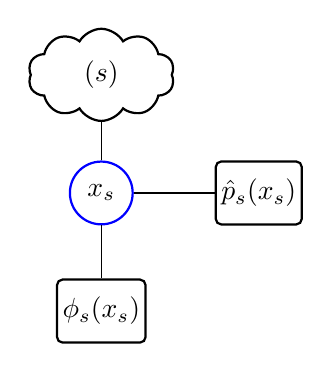
\begin{tikzpicture}
      \tikzstyle{enode} = [thick, draw=blue, circle, inner sep = 4pt,  align=center]
      \tikzstyle{nnode} = [thick, rectangle, rounded corners = 2pt,minimum size = 0.8cm,draw,inner sep = 2pt]
      \tikzstyle{cnode} = [thick, cloud, draw,cloud puffs=10, cloud puff arc=120, aspect=2, inner ysep=4pt]

      \node[cnode] (paik) at (0, 1.5) {$\Nn(s)$};
      \node[enode] (xi) at (0 ,0) {$x_s$};
      \node[nnode] (fi) at (0 , -1.5) {$\phi_s(x_s)$};
      \node[nnode] (pi) at (2, 0) {$\hat{p}_s(x_s)$};
      % connections
      \draw[-] (xi) to (fi);
      \draw[-] (xi) to (pi);
      \draw[-] (xi) to (paik);
    \end{tikzpicture}
    \caption{Factor graph illustration with prior factor.}\label{fig:factor-graph-with-prior}
    \vspace{0.1cm}
  \end{centering}
\end{figure}

As discussed in Section~\ref{sec:preliminary}, $KL(p\|q)$ is the special case of $\Dd_{\alpha}(p\|q)$ when $\alpha \rightarrow 1$. When applying $\alpha_{st}=1$, $\forall\; (s,t) \in \Ee$, to \autoref{eq:message-rule}, it gives
\begin{equation}
  {m}^{\text{new}}_{ts}(x_s) \propto \bigg[
  \sum_{x_t} \phi_{st}(x_s, x_t) {\phi}_t(x_t) \prod_{w\in \Nn(t)\backslash s}m_{wt}(x_t) \bigg],
\end{equation}
which is exactly the messages of BP in Chapter~$8$ of \cite{Bishop:2006:PRM:1162264}. From this point of view, $\alpha$-BP generalizes BP.

Inspired by \cite{pseudo_priorBP2010} and assembling methods \cite{James:2014:ISL:2517747}, we can add an extra singleton factor to each $x_v$ as prior information that is obtained from other (usually weak) methods. This factor stands for our belief from exterior estimation. Then run our $\alpha$-BP. Denote the prior by $\hat{p}_v(x_v)$ for variable node $x_v$, then the factor graph including this prior belief can be represented as in \autoref{fig:factor-graph-with-prior}.

We summarize the method into the pseudo-code in Algorithm~\autoref{alg:alphaBP}.
\begin{algorithm}
  \caption{Algorithm of $\alpha$-BP}\label{alg:alphaBP}
  \begin{algorithmic}[1]
    \renewcommand{\algorithmicrequire}{\textbf{Input:}}
    \renewcommand{\algorithmicensure}{\textbf{Output:}}
    \REQUIRE Factor graph of $p(\bm{x})$
    \STATE Initialize $q(\bm{x})$
    \IF {Prior belief on $x_i$ available}
    \STATE Add prior factor as \autoref{fig:factor-graph-with-prior}
    \ENDIF
    \WHILE{not converge}
    \FOR {each edge of factor graph}
    \STATE Message update by \autoref{eq:message-rule} or \autoref{eq:fix-factor-update}
    \ENDFOR
    \ENDWHILE
    \RETURN $q(\bm{x})$ 
  \end{algorithmic} 
\end{algorithm}

\textcolor{red}{Equivalence to EP}
\section{Convergence of $\alpha$-BP with Binary $\Aa$}
In this section we discuss the converge of $\alpha$-BP. We start from
the case binary $\Aa$ case, i.e. $\Aa=\left\{ -1, 1 \right\}$. Using the exponential potentials:
\begin{align}
  \phi_{st}(x_s, x_t) &= \exp\left\{ \theta_{st}(x_s, x_t)\right\}, \\
  \phi_{s}(x_s) &= \exp\left\{ \theta_{s}(x_s) \right\}.
\end{align}

Let us denote $\bm{\alpha}$ as the vector with entries as elements of $\left\{ \alpha_{ts} | (t ,s) \in \Ee \right\}$,  $\bm{\theta}$ as the vector with entries as elements of $\left\{ \theta_{ts} | (t ,s) \in \Ee \right\}$. Define a sized $2\abs{\Ee} \times 2\abs{\Ee}$ matrix $\bm{M}(\bm{\alpha}, \bm{\theta})$ with its entries index by edges $(t\rightarrow s)$, and of form
\begin{equation}
  M_{(t\rightarrow s), (u \rightarrow v)} =
  \begin{cases}
    \abs{ 1 - \alpha_{ts}}, &\quad u=t, v=s, \\
    \abs{ 1 - \alpha_{ts}} \tanh \abs{\alpha_{ts} \theta_{ts}}, & \quad u = s, v =t, \\
    \tanh\abs{\alpha_{ts} \theta_{ts}}, & \quad u \in \Nn(t)\backslash s, v = t, \\
    0, & \quad \mathrm{otherwise}.
  \end{cases}
\end{equation}
\begin{thm}\label{thm:normd}
  For an arbitrary pairwise Markov random field over binary variables,
  it the largest singular value of matrix $\bm{M}(\bm{\alpha}, \bm{\theta})$ is less than one,
  then $\alpha$-BP converges to a fixed point. The associated fixed
  point is unique.
\end{thm}

\begin{proof}

  Let us define the log ratio of belief on there two states:
  \begin{equation}\label{eq:log-ratio-uv}
    z_{st} = \log\frac{m_{st}(1)}{m_{st}(-1)}.
  \end{equation}
  Substituting \eqref{eq:message-rule} into \eqref{eq:log-ratio-uv} gives
  \begin{align}
    &F_{ts}(\bm{z}) = (1- \alpha_{ts})z_{ts} + \\
    &\log\frac{\exp\left\{ \alpha_{ts}\left[ \theta_{ts}(1,1) - \theta_{ts}(-1,1) \right] + \theta_t(1) - \theta_t(-1) + (1 - \alpha_{ts})z_{st} + \sum_{w\in \Nn(t)\backslash s} z_{wt} \right\}+1}
      {\exp\left\{ \alpha_{ts}\left[ \theta_{ts}(1,-1) - \theta_{ts}(-1,1) \right] + \theta_t(1) - \theta_t(-1) + (1 - \alpha_{ts})z_{st} + \sum_{w\in \Nn(t)\backslash s} z_{wt} \right\} +
      \exp\left\{ \alpha_{ts}\left[ \theta_{ts}(-1,-1) - \theta_{ts}(-1,1) \right] \right\}},
  \end{align}
  where $\bm{z}$ is vector with element entry $z_{vu}, v,u \in \Vv$.
  Further assume the symmetric property of potentials
  \begin{align}
    \theta_{ts}(x_t, x_s) &= -\theta_{ts}(x_t, -x_s) = -\theta_{ts}(-x_t, x_s), \\
    \theta_{s}(x_s) &= - \theta_s(-x_s).
  \end{align}
  With the symmetric property, the log ratio updates for $z_{ts}$ can be reduced as
  \begin{equation}\label{eq:ratio-update}
    F_{ts}(\bm{z}) = (1-\alpha_{ts}) z_{ts} + f_{ts}(\bm{z}),
  \end{equation}
  where
  \begin{equation}
    f_{ts}(\bm{z}) = \log\frac{\exp\left\{ 2 \alpha_{ts} \theta_{ts} + \Delta_{ts}(\bm{z}) \right\}+1}
    {\exp\left\{ \Delta_{ts}(\bm{z}) \right\} +
      \exp\left\{ 2 \alpha_{ts} \theta_{ts} \right\}},
  \end{equation}
  with
  \begin{equation}
    \Delta_{ts}(\bm{z}) = 2 \theta_s + (1 - \alpha_{ts}) z_{st} + \sum_{w\in \Nn(u)\backslash t} z_{wt}.
  \end{equation}

  Using $^{(n)}$ to denotes the iteration $n$. Then we have
  \begin{align}\label{eq:ratio_diff_at_n}
    z_{ts}^{(n+1)} - z_{ts}^{(n)} &= (1-\alpha_{ts}) (z_{ts}^{(n)} - z_{ts}^{(n-1)}) + f_{ts}(\bm{z}^{(n)}) - f_{ts}(\bm{z}^{(n-1)}) \nonumber \\
                                  & = (1-\alpha_{ts}) (z_{ts}^{(n)} - z_{ts}^{(n-1)}) + \nabla f_{ts}(\bm{z}^{\lambda})^{T} (\bm{z}^{(n)} - \bm{z}^{(n-1)}).
  \end{align}

  According to \cite{roosta2008reweighed_sum_product}, two functions (\textcolor{red}{to be written})
  \begin{align}
    H(\mu; \kappa) &:= \log \frac{exp(\mu + \kappa) +1}{exp(\mu) + exp(\kappa)}, \nonumber \\
    G(\mu; \kappa) &:= \frac{exp(\mu + \kappa)}{exp(\mu + \kappa) + 1} - \frac{exp(\mu)}{exp(\mu) + exp(\kappa)} = \frac{\sinh{\kappa}}{\cosh{\kappa} + \cosh{\mu}},
  \end{align}
  where it holds that
  \begin{equation}
    \pd{H(\mu; \kappa)}{\mu} = G(\mu; \kappa),
  \end{equation}
  and
  \begin{equation}
    \abs{G(\mu; \kappa)} \leq \abs{G(0, \kappa)}.
  \end{equation}

  \begin{equation}\label{eq:F_pd}
    \pd{F_{ts}(\bm{z})}{z}=
    \begin{cases}
      1 - \alpha_{ts}, &\quad z = z_{ts}  \\
      ( 1 - \alpha_{ts}) \pd{f_{ts}(\bm{z})}{\Delta_{ts}}, &\quad z = z_{st} \\
      \pd{f_{ts}(\bm{z})}{\Delta_{ts}}, &\quad z = z_{wt}, w\in N(t)\backslash s.
    \end{cases}
  \end{equation}
  Note that in \eqref{eq:F_pd}, $\pd{F_{ts}(\bm{z})}{\Delta_{ts}} = \pd{f_{ts}(\bm{z})}{\Delta_{ts}}$.

  From \eqref{eq:ratio_diff_at_n}, we have
  \begin{align}\label{eq:ratio_cvg_step}
    \abs{z_{ts}^{(n+1)} - z_{ts}^{(n)}} & = \abs{(1-\alpha_{ts}) (z_{ts}^{(n)} - z_{ts}^{(n-1)}) + \nabla f_{ts}(\bm{z}^{\lambda})^{T} (\bm{z}^{(n)} - \bm{z}^{(n-1)})} \nonumber \\
                                        & \leq \abs{(1-\alpha_{ts}) (z_{ts}^{(n)} - z_{ts}^{(n-1)})} + \abs{\nabla f_{ts}(\bm{z}^{\lambda})^{T} (\bm{z}^{(n)} - \bm{z}^{(n-1)})} \nonumber \\
                                        & = \abs{ 1 - \alpha_{ts}} \abs{z_{ts}^{(n)} - z_{ts}^{(n-1)}} + \abs{\nabla f_{ts}(\bm{z}^{\lambda})}^{T} \abs{\bm{z}^{(n)} - \bm{z}^{(n-1)}} \nonumber \\
                                        & \leq \abs{ 1 - \alpha_{ts}} \abs{z_{ts}^{(n)} - z_{ts}^{(n-1)}} + \abs{ 1 - \alpha_{ts}} \abs{G(0, 2 \alpha_{ts} \theta_{ts})} \abs{z_{st}^{(n)} - z_{st}^{(n-1)}} + \sum_{w\in N(t)\backslash s} \abs{G(0, 2 \alpha_{ts} \theta_{ts})} \abs{z_{wt}^{(n)} - z_{wt}^{(n-1)}}.
  \end{align}

  Define a sized $2\abs{\Ee} \times 2\abs{\Ee}$ matrix $\bm{M}(\bm{\alpha}, \bm{\theta})$ with its entries index by edges $(t\rightarrow s)$, and of form
  \begin{equation}
    M_{(t\rightarrow s), (u \rightarrow v)} =
    \begin{cases}
      \abs{ 1 - \alpha_{ts}}, &\quad u=t, v=s, \\
      \abs{ 1 - \alpha_{ts}} \abs{G(0, 2 \alpha_{ts} \theta_{ts})}, & \quad u = s, v =t, \\
      \abs{G(0, 2 \alpha_{ts} \theta_{ts})}, & \quad u \in \Nn(t)\backslash s, v = t, \\
      0, & \quad \mathrm{otherwise}.
    \end{cases}
  \end{equation}
  Then \eqref{eq:ratio_cvg_step} can be simplified as
  \begin{equation}\label{eq:ratio-update-ineq}
    \abs{\bm{z}^{(n+1)} - \bm{z}^{n}} \leq \bm{M}(\alpha, \bm{\theta})\abs{\bm{z}^{(n)} - \bm{z}^{n-1}},
  \end{equation}
  where $\bm{\theta}$ is the vector with elements $\left\{ \theta_{vu}| v, u \in \Vv \right\}$ and $\leq$ in \eqref{eq:ratio-update-ineq} denotes the element-wise inequality. From \eqref{eq:ratio-update-ineq}, we could have
  \begin{equation}
    \normd{\bm{z}^{(n+1)} - \bm{z}^{n}} \leq \normd{\bm{M}(\alpha, \bm{\theta})(\bm{z}^{(n)} - \bm{z}^{n-1})} \leq \lambda^{\ast}(\bm{M})\normd{\bm{z}^{(n)} - \bm{z}^{n-1}},
  \end{equation}
  where $\lambda^{\ast}(\bm{M})$ is the largest singular value of matrix
  $\bm{M}$, and $\normd{\cdot}$ is Euclidean norm. If the largest singular value of $\bm{M}$ is less than $1$, the sequence
  $\left\{\abs{\bm{z}^{(n+1)} - \bm{z}^{(n)}}\right\}$ converges to zero. Therefore, for $\lambda^{\ast}(\bm{M})<1$, the sequence $\left\{ \bm{z}^{(n)} \right\}$ is a Cauchy sequence and must converge. Let us denote vector with elements $\left\{ F_{st} \right\}$ by $\bm{F}$. $\bm{F}$ is a continuous function of $\bm{z}$. Then we have
  \begin{equation}
    \bm{F}(\lim_{n\rightarrow \infty}\bm{z}^{(n)}) = \lim_{n\rightarrow \infty}\bm{F}(\bm{z}^{(n)}).
  \end{equation}
  Assume that $\left\{ \bm{z}^{(n)} \right\}$ converges to
  $\bm{z}^{\ast}$.
  \begin{align}
    \bm{F}(\bm{z}^{\ast}) - \bm{z}^{\ast}
    &= \lim_{n\rightarrow \infty} \bm{F}(\bm{z}^{(n)}) -\lim_{n\rightarrow
      \infty} \bm{z}^{(n)} \nonumber \\
    &= \lim_{n\rightarrow \infty} (\bm{z}^{(n+1)} - \bm{z}^{(n)}) \nonumber \\
    &= 0.
  \end{align}
  Thus $\bm{z}^{\ast}$ must be a fixed point.

  In what follows we show that the fixed point is unique for $\lambda^{\ast}(\bm{M})<1$. Assume that there are two fixed points $\bm{z}_0^{\ast}$ and $\bm{z}_1^{\ast}$ for sequence $\left\{ \bm{z}^{(n)} \right\}$. Then we have
  \begin{align}\label{eq:two-fix-point}
    \bm{F}(\bm{z}_0^{\ast}) &= \bm{z}_0^{\ast}, \nonumber \\
    \bm{F}(\bm{z}_1^{\ast}) &= \bm{z}_1^{\ast}. \nonumber \\
  \end{align}
  Then
  \begin{equation}\label{eq:two-fix-ineq}
    \normd{\bm{F}(\bm{z}_0^{\ast}) - \bm{F}(\bm{z}_1^{\ast})} \leq
    \lambda^{\ast}(\bm{M})\normd{\bm{z}_0^{\ast} - \bm{z}_1^{\ast}}.
  \end{equation}
  Substituting \eqref{eq:two-fix-point} into \eqref{eq:two-fix-ineq}
  gives
  \begin{equation}\label{eq:two-fix-ineq}
    \normd{\bm{z}_0^{\ast} - \bm{z}_1^{\ast}} \leq
    \lambda^{\ast}(\bm{M})\normd{\bm{z}_0^{\ast} - \bm{z}_1^{\ast}},
  \end{equation}
  which gives us $\bm{z}_0^{\ast} = \bm{z}_1^{\ast}$.
\end{proof}

\begin{rem}
  From Theorem~\ref{thm:normd} we can see that, the sufficient condition for convergence of $\alpha$-BP is $\lambda^{\ast}(\bm{M}(\alpha, \bm{\theta})) < 1$. It is interesting to notice that $\lambda^{\ast}(\bm{M}(\alpha, \bm{\theta}))$ is a function of $\alpha$ from $\alpha$-divergence and $\bm{\theta}$. This means that whether $\alpha$-BP can converge depends on the graph $\Gg= (\Vv, \Ee)$ representing the problem itself and also the choice of $\alpha$. Therefore, proper choice of $\alpha$ can guarantee the convergence of $\alpha$-BP if the sufficient condition can possibly be fulfilled for given $\bm{\theta}$.
\end{rem}

\section{A Convergence Condition of Less Complexity for $\alpha$-BP}
Given the fact that $\alpha$-BP would converge if the condition in Theorem~\ref{thm:normd} is fulfilled, the largest singular value computation for large-sized graph could be nontrivial. Therefore, we would give a alternative sufficient condition for the convergence of $\alpha$-BP, which is easier to check compared with condition in Theorem~\ref{thm:normd}.

\begin{cor}
  $\alpha$-BP would converge if any of the following conditions is fulfilled:
  \begin{equation}
    \umax{u \rightarrow v}\abs{1-\alpha_{uv}} + \abs{1-\alpha_{vu}}\tanh{\abs{\alpha_{vu} \theta_{vu}}} + \sum_{w \Nn(v) \backslash u} \tanh{\abs{\alpha_{{vw}} \theta_{vw}}} < 1,
  \end{equation}
  or
  \begin{equation}
    \umax{t \rightarrow s} \abs{1-\alpha_{ts}} (1 + \tanh\abs{\alpha_{ts} \theta_{ts}}) + (\abs{\Nn(t)}-1)\tanh\abs{\alpha_{ts} \theta_{ts}} < 1.
  \end{equation}

\end{cor}

\begin{proof}
  From inequality~\ref{eq:ratio-update-ineq}, we can have
  \begin{align}
    \normu{\bm{z}^{(n+1)} - \bm{z}^{n}} &\leq \normu{\bm{M}(\alpha, \bm{\theta})(\bm{z}^{(n)} - \bm{z}^{n-1})}, \nonumber \\
    \normi{\bm{z}^{(n+1)} - \bm{z}^{n}} &\leq \normi{\bm{M}(\alpha, \bm{\theta})(\bm{z}^{(n)} - \bm{z}^{n-1})}.
  \end{align}
  Then we have
  \begin{align}\label{eq:row-col-norm-ineq}
    \normu{\bm{z}^{(n+1)} - \bm{z}^{n}} &\leq \normu{\bm{M}}\normu{(\bm{z}^{(n)} - \bm{z}^{n-1})}, \nonumber \\
    \normi{\bm{z}^{(n+1)} - \bm{z}^{n}} &\leq \normi{\bm{M}}\normi{(\bm{z}^{(n)} - \bm{z}^{n-1})},
  \end{align}
  where we omit the arguments of $\bm{M}$. Recall the directed-edge-indexed matrix $\bm{M}$. We can detail the two cases in \ref{eq:row-col-norm-ineq} as follows
  \begin{align}
    \normu{\bm{M}} &= \umax{u \rightarrow v}{\sum_{t\rightarrow s} M_{(t\rightarrow s), (u\rightarrow v)}} = \umax{u \rightarrow v}\abs{1-\alpha_{uv}} + \abs{1-\alpha_{vu}}\tanh{\abs{\alpha_{vu} \theta_{vu}}} + \sum_{w \Nn(v) \backslash u} \tanh{\abs{\alpha_{{vw}} \theta_{vw}}}, \nonumber \\
    \normi{\bm{M}} &= \umax{t \rightarrow s}{\sum_{u\rightarrow v} M_{(t\rightarrow s), (u\rightarrow v)}} = \umax{t \rightarrow s} \abs{1-\alpha_{ts}} (1 + \tanh\abs{\alpha_{ts} \theta_{ts}}) + (\abs{\Nn(t)}-1)\tanh\abs{\alpha_{ts} \theta_{ts}}.
  \end{align}
  When condition $\normu{\bm{M}} < 1$ is met, sequence $\{\abs{\bm{z}^{(n+1)} - \bm{z}^{n}}\}$ approaches to zero as $n\rightarrow \infty$. Similarly, condition $\normi{\bm{M}}<1$ can also guarantee the convergence to zero of sequence $\{\abs{\bm{z}^{(n+1)} - \bm{z}^{n}}\}$.
  
\end{proof}

\section{$\alpha$-BP with Local $\alpha$}
In previous sections, we have been discussing the $\alpha$-BP with a local $\alpha$ value for each factor in MRF. In this section, we would consider the case that MRF has its global $\alpha$. To be specific, when we do refinement of each factor $\phi_{st}(x_s, x_t)$ of \eqref{eq:mrf} in Section~\ref{sec:alpha-bp-factor-refine}, we use the same $\alpha$
for the problem in \eqref{eq:alpha-minimize-factor}. 
\begin{equation}\label{eq:message-rule-global}
  {m}^{\text{new}}_{ts}(x_s) \propto  m_{ts}(x_s)^{1-\alpha} \bigg[
  \sum_{x_t} \phi_{ts}(x_t, x_s)^{\alpha} {m}_{st}(x_t)^{1-\alpha} {\phi}_t(x_t) \prod_{w\in \Nn(t)\backslash s}m_{wt}(x_t) \bigg].
\end{equation}

There is a corresponding matrix
Define a sized $2\abs{\Ee} \times 2\abs{\Ee}$ matrix $\bm{M}^{\dagger}(\bm{\alpha}, \bm{\theta})$ with its entries index by edges $(t\rightarrow s)$, and of form
\begin{equation}
  M^{\dagger}_{(t\rightarrow s), (u \rightarrow v)} =
  \begin{cases}
    \abs{ 1 - \alpha}, &\quad u=t, v=s, \\
    \abs{ 1 - \alpha} \tanh\abs{ \alpha \theta_{ts}}, & \quad u = s, v =t, \\
    \tanh\abs{\alpha \theta}, & \quad u \in \Nn(t)\backslash s, v = t, \\
    0, & \quad \mathrm{otherwise},
  \end{cases}
\end{equation}


\begin{cor}\label{cor:global-alpha-bp}
  For an arbitrary pairwise Markov random field over binary variables,
  it the largest singular value of matrix $\bm{M}^{\dagger}(\bm{\alpha}, \bm{\theta})$ is less than one,
  then $\alpha$-BP converges to a fixed point. The associated fixed
  point is unique.
\end{cor}

Similar we also have the alternative sufficient condition for $\alpha$-BP with global $\alpha$ for message passing by \eqref{eq:message-rule-global}.

\begin{cor}
  $\alpha$-BP with global $\alpha$ would converge if any of the following conditions is fulfilled:
  \begin{equation}
    \umax{u \rightarrow v}\abs{1-\alpha} + \abs{1-\alpha}\tanh{\abs{\alpha \theta_{vu}}} + \sum_{w \Nn(v) \backslash u} \tanh{\abs{\alpha \theta_{vw}}} < 1,
  \end{equation}
  or
  \begin{equation}
    \umax{t \rightarrow s} \abs{1-\alpha} (1 + \tanh\abs{\alpha \theta_{ts}}) + (\abs{\Nn(t)}-1)\tanh\abs{\alpha \theta_{ts}} < 1.
  \end{equation}



\bibliographystyle{IEEEtran}

% \bibliography{bibliography}
\bibliography{myref}

% \appendix

% \input{section/sec-appendixA}
\end{document}

%%% Local Variables:
%%% mode: latex
%%% TeX-master: t
%%% End:
